% THIS IS AN EXAMPLE DOCUMENT FOR VLDB 2012
% based on ACM SIGPROC-SP.TEX VERSION 2.7
% Modified by  Gerald Weber <gerald@cs.auckland.ac.nz>
% Removed the requirement to include *bbl file in here. (AhmetSacan, Sep2012)
% Fixed the equation on page 3 to prevent line overflow. (AhmetSacan, Sep2012)

\documentclass{vldb}

\usepackage{graphicx}
\usepackage{balance}  % for  \balance command ON LAST PAGE  (only there!)

\usepackage{pdfpages}
\usepackage{fancyhdr}
\usepackage{exscale}
\usepackage{booktabs}
\usepackage{multicol}
\usepackage{multirow}
\usepackage{amsmath}
\usepackage{amsfonts}
\usepackage{amssymb}
\usepackage{rotating}
%\usepackage{afterpage,natbib,lipsum}
\usepackage{xspace}
\usepackage{afterpage,lipsum}
\usepackage{caption}
\usepackage{nicefrac}
%\usepackage{ulem}

\usepackage{times}

% \usepackage[amsthm]{ntheorem}
% \usepackage{chngcntr}
\usepackage{paralist}
\usepackage{verbatim}
\usepackage{color}
\usepackage{hyperref}
\usepackage{enumitem}
\usepackage{listings}      % source code
\usepackage{algpseudocode}
% \usepackage{algorithm}% http://ctan.org/pkg/algorithms
\usepackage{algpseudocode}% http://ctan.org/pkg/algorithmicx
\usepackage{tikz}
\usepackage{array}
\usepackage{relsize}
\usepackage{diagbox}
\usepackage{oubraces}
\usepackage{subcaption}
\usepackage{placeins}
%\usepackage{biblatex}

% \usepackage[vlined, ruled, boxed]{algorithm2e}
\usepackage[vlined,ruled]{algorithm2e}
\usepackage{xcolor}


\hbadness=1000
\tolerance=1000


\clubpenalty=500 
\widowpenalty = 1000 

%\setcounter{biburllcpenalty}{7000}
%\setcounter{biburlucpenalty}{8000}

%hack for urls
\def\UrlBreaks{\do\/\do-}

%\usepackage[maxnames=2]{biblatex}

\lstdefinelanguage{scala}{
  morekeywords={abstract,case,catch,class,def,%
    do,else,extends,false,final,finally,%
    for,if,implicit,import,match,mixin,%
    new,null,object,override,package,%
    private,protected,requires,return,sealed,%
    super,this,throw,trait,true,try,%
    type,val,var,while,with,yield},
  otherkeywords={=>,<-,<\%,<:,>:,\#,@},
  sensitive=true,
  morecomment=[l]{//},
  morecomment=[n]{/*}{*/},
  morestring=[b]",
  morestring=[b]',
  morestring=[b]"""
}
%%% optional fonts and color configuration
\SetAlFnt{\sffamily}
\renewcommand\ArgSty{\normalfont\sffamily}
\renewcommand\KwSty[1]{\textnormal{\textbf{\sffamily#1}}\unskip}
\SetAlCapFnt{\normalfont\sffamily\large}
\renewcommand\AlCapNameFnt{\sffamily\large}

\SetKwProg{Fn}{Fun}{}{}
\SetKwProg{Hdl}{Upon}{}{}

%%


% \graphicspath{{figs/}}
\newcommand{\para}[1]{\vspace{2mm}\noindent\textbf{#1}}

\definecolor{dkgreen}{rgb}{0,0.6,0}
\definecolor{gray}{rgb}{0.5,0.5,0.5}
\definecolor{mauve}{rgb}{0.58,0,0.82}


% \theoremstyle{  }

\definecolor{darkred}{rgb}{0.5,0,0}
\definecolor{darkgreen}{rgb}{0,0.5,0}
\definecolor{darkblue}{rgb}{0,0,0.5}


\newboolean{commentSwitch}

%%%%%%%%%%%%%%%%%%%%%%%%%%%%%%%%%
%% SWITCH TODOS ON/OFF HERE %%%%%
%%%%%%%%%%%%%%%%%%%%%%%%%%%%%%%%%
\setboolean{commentSwitch}{true}
%%%%%%%%%%%%%%%%%%%%%%%%%%%%%%%%%
%%%%%%%%%%%%%%%%%%%%%%%%%%%%%%%%%

\ifthenelse{\boolean{commentSwitch}}{
  \newcommand{\kostas}[1]{\textcolor{blue}{Kostas: #1}}
  \newcommand{\stephan}[1]{\textcolor{darkred}{Stephan: #1}}
  \newcommand{\paris}[1]{\textcolor{purple}{Paris: #1}}
  \newcommand{\gyula}[1]{\textcolor{darkgreen}{Gyula: #1}}
  \newcommand{\stefan}[1]{\textcolor{brown}{Stefan: #1}}
  
  \newcommand{\TODO}[1]{\textcolor{red}{TODO: #1}}
  \newcommand{\TODOP}[1]{\textcolor{red}{TODO: #1}}
  \newcommand{\TODOX}[1]{\textcolor{red}{TODO: #1}}
  \newcommand{\NOTE}[1]{\textcolor{blue}{\textbf{NOTE}: #1}}
  \newcommand{\DONEX}[1]{\textcolor{blue}{#1}}
}{
  \newcommand{\kostas}[1]{}
  \newcommand{\stephan}[1]{}
  \newcommand{\paris}[1]{}
  \newcommand{\gyula}[1]{}
  \newcommand{\stefan}[1]{}
  \newcommand{\TODO}[1]{}
  \newcommand{\NOTE}[1]{}
}

\newcommand{\wip}[1]{\textcolor{red}{WIP: #1}}
\newcommand{\Tau}{\ensuremath{\mathcal{T}}}
\newcommand{\Rev}[2]{\textcolor{red}{\textbf{R-#1}:#2}}

\lstset{frame=l,
  language=Java,
  aboveskip=3mm,
  belowskip=3mm,
  showstringspaces=false,
  xleftmargin=5pt,
%   framexleftmargin=-1pt,
  columns=flexible,
  basicstyle={\scriptsize\ttfamily},
  numbers=none,
  numberstyle=\tiny\color{black},
  keywordstyle=\color{blue},
  commentstyle=\color{dkgreen},
  stringstyle=\color{mauve},
  breaklines=true,
  breakatwhitespace=true,
  tabsize=4,
  %for scala
  emph={%  
    object, def, val, zip, window, trigger, evict%
    },emphstyle={\color{blue}\textbf}%
}%


% \usepackage[
% % backend=biber
% % style=alphabetic,
% % sorting=abbrv
% ]{biblatex}

% \renewbibmacro{in:}{}

 
% \addbibresource{references.bib}
% \renewcommand{\bibfont}{\small} % or any other  appropriate font command

% url references
% \usepackage[hidelinks]{hyperref}

% % in paragraph enums
% \usepackage{paralist}

% \usepackage{subfig}

\def\definitionautorefname{Definition}
\def\sectionautorefname{Section}
\def\subsectionautorefname{Section}
\def\subsubsectionautorefname{Section}
\def\algorithmautorefname{Algorithm}
\def\figureautorefname{Figure}

\begin{document}

% ****************** TITLE ****************************************

\title{State Management in Apache Flink\textsuperscript{\textregistered}}

\subtitle{Consistent Stateful Distributed Stream Processing}
% possible, but not really needed or used for PVLDB:
%\subtitle{[Extended Abstract]
%\titlenote{A full version of this paper is available as\textit{Author's Guide to Preparing ACM SIG Proceedings Using \LaTeX$2_\epsilon$\ and BibTeX} at \texttt{www.acm.org/eaddress.htm}}}

% ****************** AUTHORS **************************************

% You need the command \numberofauthors to handle the 'placement
% and alignment' of the authors beneath the title.
%
% For aesthetic reasons, we recommend 'three authors at a time'
% i.e. three 'name/affiliation blocks' be placed beneath the title.
%
% NOTE: You are NOT restricted in how many 'rows' of
% "name/affiliations" may appear. We just ask that you restrict
% the number of 'columns' to three.
%
% Because of the available 'opening page real-estate'
% we ask you to refrain from putting more than six authors
% (two rows with three columns) beneath the article title.
% More than six makes the first-page appear very cluttered indeed.
%
% Use the \alignauthor commands to handle the names
% and affiliations for an 'aesthetic maximum' of six authors.
% Add names, affiliations, addresses for
% the seventh etc. author(s) as the argument for the
% \additionalauthors command.
% These 'additional authors' will be output/set for you
% without further effort on your part as the last section in
% the body of your article BEFORE References or any Appendices.

%\numberofauthors{6} 

%ordered by last name
\numberofauthors{3}
\author{
\alignauthor Paris Carbone\textsuperscript{$\dagger$} \alignauthor Stephan Ewen\textsuperscript{$\ddagger$} \alignauthor Gyula F\'ora\textsuperscript{$\star$} \and \alignauthor Seif Haridi\textsuperscript{$\dagger$} \alignauthor Stefan Richter\textsuperscript{$\ddagger$} \alignauthor Kostas Tzoumas\textsuperscript{$\ddagger$} \and
\\
\begin{tabular}{*{3}{>{\centering}p{.31\textwidth}}}
\affaddr{\textsuperscript{$\dagger$}KTH Royal Institute of Technology} \\ \affaddr{\{parisc,haridi\}@kth.se} & \affaddr{\textsuperscript{$\star$}King Digital Entertainment Limited} \\ \affaddr{gyula.fora@king.com} & \affaddr{\textsuperscript{$\ddagger$}data Artisans} \\ \affaddr{\{stephan,s.richter,kostas\} \\@data-artisans.com}
\end{tabular}
}
\vspace{-5mm}

%\author{
%}

% \alignauthor
% Ben Trovato\titlenote{Dr.~Trovato insisted his name be first.}\\
%       \affaddr{Institute for Clarity in Documentation}\\
%       \affaddr{1932 Wallamaloo Lane}\\
%       \affaddr{Wallamaloo, New Zealand}\\
%       \email{trovato@corporation.com}
% % 2nd. author
% \alignauthor
% G.K.M. Tobin\titlenote{The secretary disavows
% any knowledge of this author's actions.}\\
%       \affaddr{Institute for Clarity in Documentation}\\
%       \affaddr{P.O. Box 1212}\\
%       \affaddr{Dublin, Ohio 43017-6221}\\
%       \email{webmaster@marysville-ohio.com}
% % 3rd. author
% \alignauthor Lars Th{\Large{\sf{\o}}}rv{$\ddot{\mbox{a}}$}ld\titlenote{This author is the
% one who did all the really hard work.}\\
%       \affaddr{The Th{\large{\sf{\o}}}rv{$\ddot{\mbox{a}}$}ld Group}\\
%       \affaddr{1 Th{\large{\sf{\o}}}rv{$\ddot{\mbox{a}}$}ld Circle}\\
%       \affaddr{Hekla, Iceland}\\
%       \email{larst@affiliation.org}
% \and  % use '\and' if you need 'another row' of author names
% % 4th. author
% \alignauthor Lawrence P. Leipuner\\
%       \affaddr{Brookhaven Laboratories}\\
%       \affaddr{Brookhaven National Lab}\\
%       \affaddr{P.O. Box 5000}\\
%       \email{lleipuner@researchlabs.org}
% % 5th. author
% \alignauthor Sean Fogarty\\
%       \affaddr{NASA Ames Research Center}\\
%       \affaddr{Moffett Field}\\
%       \affaddr{California 94035}\\
%       \email{fogartys@amesres.org}
% }

% There's nothing stopping you putting the seventh, eighth, etc.
% author on the opening page (as the 'third row') but we ask,
% for aesthetic reasons that you place these 'additional authors'
% in the \additional authors block, viz.

% \additionalauthors{Additional authors: John Smith (The Th{\o}rv\"{a}ld Group, {\texttt{jsmith@affiliation.org}}), Julius P.~Kumquat
% (The \raggedright{Kumquat} Consortium, {\small \texttt{jpkumquat@consortium.net}}), and Ahmet Sacan (Drexel University, {\small \texttt{ahmetdevel@gmail.com}})}
% \date{30 July 1999}

% Just remember to make sure that the TOTAL number of authors
% is the number that will appear on the first page PLUS the
% number that will appear in the \additionalauthors section.

\maketitle

\begin{abstract}
Stream processors are emerging in industry as a paradigm that drives analytical but also mission critical services that encapsulate the core of persistent application logic. Thus, apart from low-latency, an emerging need is to provide first-class support for application state together with strong consistency guarantees and fast adaptivity to cluster reconfigurations, software patches and partial failures. Prior systems research has addressed some of these problems. However, the practical challenge lies on how such guarantees can be materialized in a transparent, non-intrusive manner that relieves the user from unnecessary constraints.
%\stefan{This statement basically sets it in the focus of the paper's contribution. I suggest that for each part, you particularly get back to how the implementation is transparent, non-intrusive and free of constraints.} 
Such needs served as the main design principles of state management in Apache Flink\textsuperscript{\textregistered}, an open source, scalable stream processor. 

At Flink's core, an asynchronous in-band, snapshotting mechanism guarantees the creation of lightweight, consistent, distributed snapshots of application state, progressively without impacting continuous progress. Consistent snapshots cover all needs for system reconfiguration, fault tolerance and version management through coarse grained rollback recovery. Application state is declared explicitly to the system, allowing efficient partitioning and transparent commits to persistent storage. We further present Flink's backend implementations, and mechanisms for high availability and output commit. Finally, we demonstrate how these mechanisms behave in practice with metrics and large-deployment insights exhibiting the low performance trade-offs of our approach and the general benefits of exploiting asynchrony in continuous, yet sustainable system deployments.

\end{abstract}


%!TEX root = main.tex

\section{Introduction}
\label{sec:intro}

Traditionally, when implementing data-driven applications and services, \emph{state} was separated from the application logic that performs the computation on data. The typical architecture has the state centralized in a database management system shared among applications that are either stateless or, rely on the database for data consistency and scalability among others.

Recently, stream processing has been gaining tremendous attention in the industry as a paradigm to implement both analytical applications on "real-time" data, but also as a paradigm to implement data-driven applications and services that would otherwise interact with an operational database for their data access needs. The stream processing paradigm is more friendly to modern organizations that separate engineering teams vertically, each team being responsible for a specific feature or application, as it allows state to be distributed and co-located with the application instead of forcing teams to collaborate by sharing access to an operational database. Further, stream processing is a natural paradigm for \emph{event-driven} applications that need to react fast to real-world events and communicate with each other via message passing. 

In point of fact, stream processing is not a new concept; it has been an active research topic for the database community in the past \cite{chen2000niagaracq,cherniack2003scalable,chandrasekaran2003telegraphcq,abadi2003aurora,arasu2004stream} and some (but not all) of the ideas that underpin modern stream processing technology are inspired by that research. However, what we see today is widespread adoption of stream processing across the enterprise beyond niche applications where stream processing and Complex Event Processing systems were traditionally used. There are many reasons for this: first, new stream processing technologies allow for massive scale-out similar to MapReduce \cite{dean2008mapreduce} and related technologies \cite{zaharia2010spark,stratosphere,battre2010nephele}. Second, the amount of data that is generated in the form of event streams is exploding. Processing needs now spread beyond financial transactions, to user activity in websites and mobile apps, as well as data generated by machines and sensors in manufacturing plants, cars, home devices, etc. Third, many modern state of the art stream processing systems are open source allowing widespread adoption in the developer community. 

Earlier attempts to distributed stream processing \cite{CUSTOM:web/Storm} provided distributed programming model semantics but focused on the challenge of producing real-time, perhaps approximate results that would later be augmented or corrected by more reliable, periodic (e.g., overnight) batch compute jobs (e.g., Lambda Architecture \cite{marz2015big}). While this addresses real-time compute on data records most challenges related to consistent state management remain a concern of the user and typically rest upon external database management systems or traded off for further scalability.

%- What is the problem?
%Data stream processing has been traditionally decoupled from database management systems. When it comes to continuous data processing technologies, stream processors, have been viewed as a secondary tool for generating approximate, often inconsistent results in a timely manner. Recent advances in data streaming technologies have focused on providing distributed programming model semantics \cite{CUSTOM:web/Storm,CUSTOM:web/Samza} that can address large scale data ingestion, to deal with increasing data volumes. While this enables a new variety of applications, challenges related to consistent state management remain a concern of the user and are typically lifted to external database management systems or traded off for further scalability (e.g. Lambda Architecture \cite{marz2015big}).

We identified a set of hard challenges, faced daily by developers that architect critical continuous applications in the real world. First, the lack of explicit computational state abstractions in stream processing systems forces them to declare and maintain state externally, decoupled from computational logic. Hence, the burden of ensuring data consistency lies in the application logic, coordinating computation with external database systems. Often, this is complex to maintain as the code-base is divided across the state it manages. Second, transactions with external storage can become the bottleneck of the whole application. Finally, operational challenges arise when there is need to scale in or out, deal with partial failures or to simply change application logic with software patches. While several of these important state management issues have been previously researched and applied in production systems, most known approaches fall short of doing so in a transparent manner. For example, micro-batching techniques for reliable continuous processing (e.g. Apache Spark and Trident \cite{zaharia2012discretized,CUSTOM:web/trident}) sacrifice programming model transparency and processing latency by enforcing batch-centric application logic. Other proprietary continuous processing system solutions \cite{millwheel} on the other hand, build on heavy transactional per-record processing. This pushes critical complexities outside the system relying on high-performance key-value stores, special hardware and optimized network infrastructure. 

Apache Flink \cite{CUSTOM:web/Flink} is a stream processing system that addresses these challenges by closely integrating state management with computational logic. Flink's dataflow execution encapsulates distributed, record-centric operator logic to express complex data pipelines. Consistent application state is a first-class citizen in data processing pipelines written in Flink and is persisted using a modular state backend. Furthermore, the system manages operations on state and orchestrates failure recovery and reconfiguration (scale-out/in) whenever necessary without imposing heavy impact on the execution or violating consistency. 
%Pipeline output committed to external databases or distributed file systems respects standard isolation level guarantees that have been traditionally supported by transactional databases such as ``read-committed'' or ``read-uncommitted'' application state. 
The core of our approach in Apache Flink builds on \emph{distributed snapshots}, a  classical concept that is proliferating anew today. Distributed snapshots enable rollback recovery of arbitrary distributed processes \cite{elnozahy2002survey} to a prior globally consistent execution state. Several distributed computing systems have used different variations of snapshotting mechanisms \cite{murray2013naiad,low2012distributed}, though adopting sub-optimal protocols that impose global synchrony and thus halt computational progress while also persisting more state than required (i.e. records within network buffers).

%\stephan{Two comments on the last sentence: (1) State is not necessary "local", but may very well be remote. I think what you mean here is state that looks as if it is local and is used similar to operator-local state. Flink actually does not make the assumption that state is local (see Gyula's MySQL state backend) and the new DataFlow runner (as a service on Google Cloud) for Beam uses BigTable as a service to store state - hence state is remote. I would simply write here "Such operators typically maintain state and exchange ...". Local state is already a design choice of Flink. (2) I would personally completely drop the term "user defined function" or making any form of distinction between operators and user-functions - that is more confusing then helpful to the reader. Everything is operators. Whether they execute built-in functions, user-defined functions, or code generated from higher declarative abstractions really does not matter.}

%\stephan{This sections again is written under the specific assumption of local partitioned state, and it implicitly assumes that this is the common default model. I would assume that actually the opposite is true - most people come from a mental model of state and computation being separate: A computing system (stream processor) and a state system (database), where the computing system operates against the storage system. That is what most companies have implemented in their Infrastructure. The challenges you highlight are actually somewhat trivial in that model - re-scaling (at least of the computation) and applying patches happens on stateless containers, which makes it very simple.}

%- Why is it interesting and important?
%- Why is it hard? (E.g., why do naive approaches fail?)


%Why hasn't it been solved before? (Or, what's wrong with previous proposed  solutions? How does mine differ?)
%What are the key components of the approach and results? Also include any specific limitations.

In this work, we present a complete, continuous state management solution that builds on distributed snapshots. Flink's snapshotting mechanism has been in use since version 0.9 (June 2015) and therefore hardened throughout frequent releases of the framework and extensively tested in production at some of the largest stream processing deployments in the world, on 1000s of nodes  managing hundreds of gigabytes of state (see \autoref{sec:evaluation}). 
%\stephan{I would drop the 'Alibaba' in the text, just reference the cluster. A foot note may be okay instead.}
The state snapshotting mechanism is coordinated and pipelined, similarly to the classical Chandy-Lamport's protocol \cite{chandy1985distributed}. However, it is fine-tailored for weakly connected dataflow graphs to superimpose the acquisition of consistent snapshots without heavily impacting throughput. More importantly, snapshots are compacted, limited to minimal computational state with the exception of cyclic dataflow graphs where the partial inclusion of records in-transit is necessary. In situations where relaxed processing guarantees are acceptable (i.e. at-least once processing guarantees) a totally asynchronous version of the protocol can be selected on-demand. 
Moreover, state and output that can be accessed from outside the system (e.g. queryable state, pipeline output) is provided under different isolation levels (read committed or uncommitted) in order to satisfy the required trade off between consistency and latency. 
This paper is the first principled description of the techniques that are implemented in Apache Flink for state management. The main goal of this work is to accurately describe these techniques and their significance\footnote{Most authors have been involved in the conception and implementation of these core techniques. Yet, the full credit for the evolution of Flink's ecosystem goes to the Apache Flink community, currently having more than 250 contributors.}. To summarize, this paper's contributions:

\begin{itemize}
	\item We tailor state snapshotting to the needs of typical distributed stream processing pipelines on common, weakly connected dataflow graphs.
	\item We provide a complete end-to-end design for continuous stateful processing, from the conceptual view of state in the programming model to its physical counterpart implemented in various backends.
	\item We encapsulate different processing guarantees and isolation levels for accessing partitioned operator state and output, using snapshots.
	\item We demonstrate how snapshots can be utilized for a large variety of operational needs beyond failure recovery such as software patches, testing, system upgrades and rescaling.
	\item We describe live, large-scale pipeline production deployments that operate 24/7 in production and rely heavily on stateful processing coupled with runtime metrics and performance insights.
\end{itemize}

The rest of the paper is organized as follows: \autoref{sec:preliminaries} gives an overview of the Apache Flink stack and the basic principles behind distributed snapshots and guarantees for dataflow execution graphs. In \autoref{sec:core} we describe the core state management mechanisms of Flink, namely its stateful programming abstractions, the snapshotting protocol and its practical usages. \autoref{sec:implementation} summarizes further implementation concerns such as backend support, concurrent snapshots, the ability to query application state as well as end-to-end guarantees. Finally, \autoref{sec:evaluation} describes existing large-scale deployments and discusses metrics related to Flink's snapshots, followed by related work in \autoref{sec:related} and our conclusions coupled with future work and acknowledgements summarized in \autoref{sec:conclusion}. 

\balance
%!TEX root = main.tex

\begin{figure*}[t!]
\centering
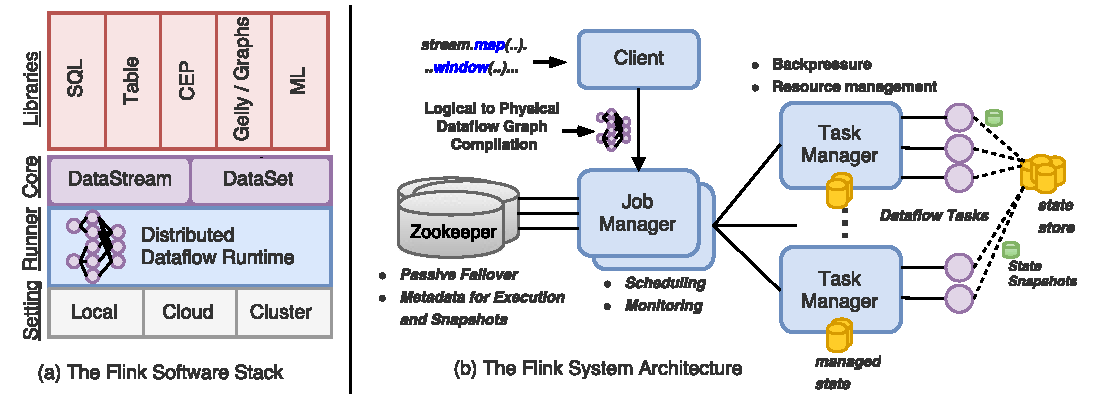
\includegraphics[width=\textwidth]{figures/flinkoverview.pdf}
\caption{An Overview of the Apache Flink System Model and Architecture.} 
\label{fig:flink-overview}
\vspace{-4mm}
\end{figure*}

\section{Preliminaries}
\label{sec:preliminaries}
\subsection{The Apache Flink System}

The Apache Flink system \cite{CUSTOM:web/Flink} is an open-source project that provides a full software stack for programming, compiling and running distributed continuous data processing pipelines (\autoref{fig:flink-overview}(a)). Pipelines can be written as a series of data-centric transformations expressed in a fluid, functional programming API (in Scala, Java or Python) inspired by Flume Java\cite{chambers2010flumejava}, Dryad LINQ\cite{yu2008dryadlinq}, Naiad\cite{murray2013naiad} and the Dataflow Model \cite{akidau2015dataflow}. At the core of the model there are two basic abstract data types, the \emph{DataSet} and \emph{DataStream} representations which target bounded and unbounded datasets respectively. Computation declared using the available higher-level domain-specific libraries such as the SQL and Machine Learning (ML) packages, in fact, translates into a logical pipeline using these core representations. A major distinctive trait of the Flink programming model compared to state of the art is the capability to declare local or partitioned, persistent application state within continuous user-defined transformations through managed data collections with diverse properties (append-only, mutable, etc.). Flink's runtime ensures that consistency is guaranteed for any managed state declared despite potential partial failures or reconfiguration periods.

Logical pipeline representations are optimised and mapped to physical graphs of dataflow operators encapsulating the user-defined logic at the client side. Physical graph representations are shipped to Flink's runtime, a continuous dataflow execution environment which deploys and manages their continuous execution as depicted in \autoref{fig:flink-overview}(b). As with most distributed data processing systems, there is a \emph{JobManager}, a master process that holds the metadata of active pipelines and coordinates execution by communicating with worker processes, the TaskManagers. Communication between the the JobManager and TaskManagers respects an asynchronous RPC-based communication protocol, consisting of periodic status updates (heartbeats) to the JobManager and scheduling requests back to the TaskManagers. In contrast to batch-centric job management \cite{zaharia2012discretized,venkataramandrizzle} which prioritizes reconfiguration and coordination, Flink employs a schedule-once, long-running allocation of tasks. However, the system is flexible to trivially reconfigure pipelines to more or less workers and re-allocate application state on-demand. This approach minimizes management overhead while allowing for fast adaptation to hardware or software changes or partial failures that can potentially occur. Finally, pipeline deployments in Flink are highly available, thus, tolerating even master failures via leader election and passive failover in Zookeeper. All underlying mechanisms for state partitioning, snapshotting and maintenance are the main focus and covered thoroughly in this paper.


\subsection{Distributed Snapshots}

Distributed systems are typically designed to mask away from the user or programmer concerns related to their distributed nature, thus, offering the view of a single entity. For a distributed data computing system like Flink we often have to reason about the state of a distributed pipeline in production at any time during its computation. Knowing and referring to the complete state of a computation as an atomic unit is essential since we can use it to correctly rollback the full computation to the point in time when that state was captured, a common case when reconfiguration is required or a partial failure caused a violation of the correct execution of the pipeline. This approach is also known as rollback recovery \cite{elnozahy2002survey}. Distributed snapshotting \cite{chandy1985distributed} protocols enable rollback recovery by producing a correct state replica of a distributed execution which can be therefore used to restore a system back to a specific point in time. In the context of a graph of dataflow tasks the execution state at any time 

\paris{we should simply explain exactly once processing guarantees, consistency and briefly mention what is the SoA}


%!TEX root = main.tex

\section{Core Concepts and Mechanisms}
\label{sec:core}

\subsection{System Model}

Each processing pipeline in Flink is first defined as a logical directed graph $G = (\mathcal{T}, \mathcal{E})$ where $\mathcal{T}$ is a set of vertices representing compute tasks and $\mathcal{E}$ is a set of edges representing data subscriptions between tasks in $\mathcal{T}$ (\autoref{fig:graphs}(a)). Data subscriptions can apply arbitrarily between tasks in $\mathcal{T}$, addressing the dependencies prescribed directly or indirectly via the programming model (e.g., forward, shuffle and hash partitioning). A task $t \in \mathcal{T}$ can encapsulate the logic of a single operation (e.g., \texttt{map}, \texttt{filter}, \texttt{fold}, \texttt{window}). However, standard logical dataflow optimisations  such as fusion \cite{hirzel2014catalog,chambers2010flumejava} are also applied in an intermediate step allowing multiple operators to share the same task in $\mathcal{T}$ (\autoref{fig:graphs}(b)). Each logical graph is directly mapped to a physical, distributed graph $G^*$ upon deployment or rescaling (\autoref{fig:graphs}(c)). In the rest of this section we are going to introduce the concept of managed state in Apache Flink, followed by physical state partitioning and a description of how state and data are being allocated to tasks.

\begin{figure}[t]
\centering
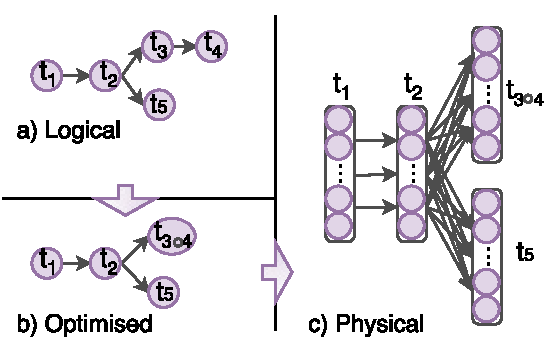
\includegraphics[width=\textwidth / 2]{figures/graphs.pdf}
\vspace*{-5mm}
\caption{Dataflow Graph Representation Examples.} 
\label{fig:graphs}
\vspace{-2mm}
\end{figure}

\subsubsection{Managed State}
\label{sec:managedstate}
Each stream operation in Flink can declare its own state and update it continuously in order to maintain a summary of the data seen so far. State is a main building block of a pipeline as it encapsulates, at any time, the full status of the computation. There are conceptually two scopes upon which managed state operates. For purely data-parallel stream operations such as a per-key average, the computation, its state and associated streams can be logically scoped and executed independently for each key. This is similar to how a relational \texttt{GROUP\_BY} projects rows of the same key to the same set to compute grouped aggregates. We refer to this state as \texttt{Keyed-State}.
For local per-task computation such as a partial machine learning training model, state can be declared in the level of a parallel physical dataflow task, known as \texttt{Operator-State}. Both \texttt{Keyed-State} and \texttt{Operator-State} are transparently partitioned and managed by the runtime of the system. More importantly, the system can guarantee that update operations on managed state will be reflected exactly-once with respect to the input streams. In \autoref{sec:implementation} we explain in detail how the file system facilitates efficient external state persistence of different state types despite the local view exposed to the programmer. Below, we briefly explain how managed state can be declared and the basic intuition for each of the state types. 

%\stephan{I think we should write "he system can guarantee that update operations on managed  state  will be REFLECTED exactly-once with respect to the input streams. That more accurately captures the approach of rollback plus replay.}

\para{\texttt{Keyed-State}}: Any data-parallel stream computation can be mapped to a user-defined key space and as a result any associated state will also be scoped together with the computation. Typically, data-stream records arrive to the system with some domain-specific key such as a user-session identifier, a device address or a geographical location. In the most general case, Flink allows for a user to map any record from its schema domain $\mathcal{S}$ to a given key space $\mathcal{K}$ via the $\texttt{keyby}: \mathcal{S} \rightarrow \mathcal{K}$ operation supported by the \texttt{DataStream} abstract type. Under key scope, state can be allocated dynamically within a user-defined function by using special collections that the model exposes through the API and vary depending on the nature of the state. For append-only state per key (e.g. for storing a pattern sequence or a window) there is a \texttt{ListState} collection supporting an \texttt{add} operation. If  the state is otherwise a value that mutates during the application logic, there is a \texttt{ValueState} type supporting an \texttt{update} operation. Other basic state types such as \texttt{ReduceState} further allow for one or two-step, on-the-fly, distributive function aggregations on managed state. Finally, the \texttt{MapState} state type can support \texttt{put} and \texttt{get} key-value operations and is preferred over having a custom map declared as a \texttt{ValueState} since it avoids a full map deserialization to perform single key lookups.

\para{\texttt{Operator-State}}: Another scope upon which state and computation can be declared is within the granularity of each parallel instance of a task (task-parallel). \texttt{Operator-State} is used when part of a computation is only relevant to each physical stream partition, or simply when state cannot be scoped by a key. A Kafka ingesting source operator instance for example that has to keep offsets to respective partitions in Kafka \cite{kreps2011kafka} is using this scope. \texttt{Operator-State} adheres to a \emph{redistribution pattern} that allows breaking state into finer-grained units when possible, allowing the system to redistribute state when changing the parallelism of the operator (scale in/out).
%In cases where \texttt{Operator-State} state can be further divided into finer-grained units (e.g., in Kafka-ingesting data sources when each task instance has to keep track of multiple partitions in Kafka)


%the \texttt{ListState} type can be used to declare further state units. Both \texttt{Keyed-State} and \texttt{Operator-State} scopes can be used in combination within a single user-defined operator on Flink, allowing for multiple granularities to handle state and processing-logic.

%\stephan{I think a reference to ListState it hard to get for an unfamiliar reader. How about writing something like this: "Operator-State typically declares a "redistribution pattern" that described how to break the state into finer-grained units and how to redistribute state when changing the parallelism of the operator (scale in/out)."}

%such as the source instances of a pipeline that correspond to Kafka consumers that map an active offset per partition
%Operator-state types are similar to Keyed-State (i.e., \texttt{ListState}, \texttt{ValueState}), whereas
%, both scopes 


%\stefan{The last sentence is partially incorrect. Right now, there is only list state for operator state, but it is also semantically different. It resembles more a value state and the only purpose of providing it in a list is breaking it down to repartitionable units for rescaling. Before rescaling was introduced, this state was just one huge black box, and Flink could never reason about how to redistribute this. Now, the user can divide the state into multiple black boxes. While they are still opaque for Flink, the system is now free to redistribute them.}

\begin{figure*}[t]
\centering
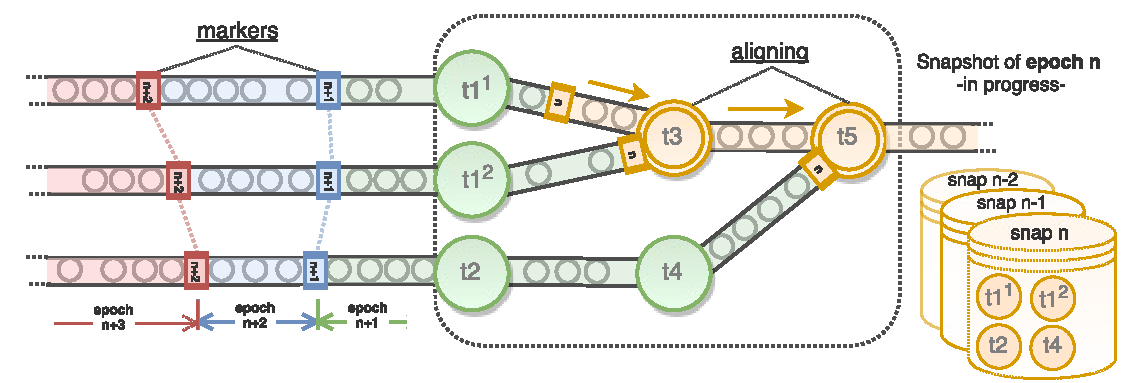
\includegraphics[width=\textwidth]{figures/snapshots-overview.pdf}
\vspace*{-10mm}
\caption{An Example of the Pipelined Snapshotting Protocol.} 
\label{fig:snapshots-overview}
\vspace{-2mm}
\end{figure*}


\subsubsection{State Partitioning and Allocation}

\para{Physical Representation}: The mapping of a logical graph $G$ to $G^* = \{\mathcal{T^*}, \mathcal{E^*}\}$, the physical, distributed execution graph (\autoref{fig:graphs}(c)) occurs when a pipeline is deployed, on its initial run or upon reconfiguration (e.g., for scale-out). During that stage each logical task $t \in \mathcal{T}$ is mapped to a number of physical tasks $t^1, t^2, \ldots, t^\pi \in \mathcal{T^*}$, each of which gets deployed to available containers throughout a cluster (e.g., using YARN \cite{vavilapalli2013apache} or Mesos \cite{hindman2011mesos}) up to the decided degree of parallelism $\pi \in \mathbb{N^+}$. 

\para{Key-Groups}: For tasks that have declared managed keyed state, it is important to consistently allocate data stream partitions or re-allocate in the case of reconfiguration. For flexibility, Flink decouples key-space partitioning and state allocation similarly to Dynamo\cite{decandia2007dynamo}. Consider a user-defined key space $\mathcal{K}$. The runtime maps keys to an intermediate circular hash space of ``key-groups'' : $\mathcal{K}^* \subset \mathbb{N^+}$ given a maximum parallelism $\pi\text{-max}$ and a hash function $h$ as such:

\noindent $\mathcal{K}^* = \{ h(k)\text{ \texttt{mod} }\pi\text{-max}\text{ }|\text{ }k \in \mathcal{K}, \pi\text{-max} \in \mathbb{N^+}, h: \mathcal{K} \rightarrow \mathbb{N^+} \}$

\noindent This mapping ensures that a single parallel physical task will handle all states within each assigned group, making a key-group the atomic unit for re-allocation. The intuition behind key-groups lies in the trade-off between reconfiguration time (I/O during state scans) and metadata needed to re-allocate state (included within snapshots). On one extreme each parallel task could scan the whole state (often remotely) to retrieve the values of all keys assigned to it. This yields significant amounts of unnecessary I/O. 
%\stephan{("sequential" does not really add anything here. It is also not really guaranteed that this is always sequential, as the blob storage for the checkpoints can be a whatever. I would drop that term.)}  
On the opposite extreme, snapshots could contain references to every single key-value and each task could selectively access its assigned keyed states. However, this approach increases indexing costs (proportional to num. of keys) and communication overhead for multiple remote state reads, thus, not benefiting by coarse-grained state reads. Key-groups offer a substantial compromise: reads are only limited to data that is required and key-groups are typically large enough for coarse grained sequential reading (if $\pi\text{-max}$ is set appropriately low). In the uncommon case where $|\mathcal{K}| < \pi\text{-max}$ it is possible that some task instances simply receive no state.

%\stephan{This reads very "local disk" centric, where one optimizes for "sequential vs. random I/O". Is that the correct general terminology when talking about accessing data (remotely)? We could also use the terms "coarse grained" state access (reading/fetching a lot of unnecessary data) versus "many fine grained accesses" where the per-request overhead (remote request plus seek) makes it extremely expensive.}

\para{State Re-Allocation}: To re-assign state, we employ an equal-sized  key-group range allocation. For $\pi$ parallel instances, each instance $t^i \in \mathcal{T^*}, 0\leq i \leq \pi$ receives a range of key-groups from $\lceil i \cdot \frac{\pi\text{-max}}{\pi} \rceil$ to $\lfloor (i+1) \cdot \frac{\pi\text{-max}}{\pi} \rfloor$. Seeks are costly, especially in distributed file systems. Nevertheless, by assigning contiguous key-groups we eliminate unnecessary seeks and read congestion, yielding low latency upon re-allocation. 
\texttt{Operator-State} entries, which cannot be scoped by a key, are persisted sequentially (combining potential finer-grained atomic states defined across tasks), per operator, within snapshots and re-assigned based on their \emph{redistribution pattern}, e.g., in round-robin or by broadcasting the union of all state entries to all operator instances. \\
%Stephan: I think that is enough on the conceptual level - no need to go into more details here (it becomes very implementation specific otherwise).

%\stefan{You could use the black-box explanation that I mentioned in earlier comments. Operator-state is simply reassigned in round-robin, aiming to balance the number of assigned states among all tasks as much as possible. Additionally, we also have features called global and broadcast state. It is fully implemented, but currently not exposed in public API. This feature is based on replicating operator state from one task to all tasks upon restart, where replication means that all receiver read this from the same source, they just get a handle. In global state, we do a one-to-all replication (initially only one task has this task, upon restart it is replicated to all tasks), in broadcast state, we do all-to-all. }

\subsection{Pipelined Consistent Snapshots}
\label{sec:snapshots}

Flink's snapshotting protocol provides a uniform way to capture the complete state of a pipeline and roll it back whenever that is required. We will first explain its intuition followed by a more formal definition of the assumptions and description of the protocol for directed acyclic and cyclic graphs respectively.


\subsubsection{Approach Intuition}

A continuous stream execution is conceptually divided into logical periods that ``cut'' a distributed data stream into consecutive finite sets of records (\autoref{fig:snapshots-overview}), which we call \emph{epochs}. An \emph{epoch} can be triggered on-the-fly, periodically by the system or on-demand by the user and is decoupled from any application logic (e.g., windowing constrains). A snapshot of the computation at \emph{epoch} $n$ refers to a copy of the internal state of each task $t \in \mathcal{T^*}$ after the system fully ingests every input record from the beginning of the computation (\emph{epoch} 0) up to and including \emph{epoch} $n$. In case of a failure during or before a snapshot of \emph{epoch} $n$ is acquired we can simply revert the global state of the distributed dataflow graph to a previous \emph{epoch} (e.g., $n-1$). A discrete approach to snapshotting would be to let the system fully ingest \emph{epoch} $n$, log the internal state of each task $t \in \mathcal{T^*}$ and then proceed with \emph{epoch} $n+1$ (similarly to micro-batching \cite{zaharia2012discretized}). However, this approach raises latency and underutilization costs related to the coordination of a discrete execution which can be hard to amortize. Furthermore, other protocols either disrupt normal execution \cite{murray2013naiad,jacques2016consistent} or are incapable of supporting typical weakly connected graphs \cite{chandy1985distributed}.

Instead, Flink's snapshotting protocol pipelines progressively the partial acquisition of task states to eventually acquire a complete snapshot, respecting \emph{epochs}, while running concurrently alongside normal operation. Special markers are injected in each data stream partition at the dataflow sources, coordinated by the runtime and get disseminated throughout the dataflow graph as depicted in \autoref{fig:snapshots-overview}. Markers signal distributed tasks of new epochs and thus aid to establish the appropriate moment to snapshot each local state and proceed with further processing promptly. Tasks with multiple inputs execute an \emph{alignment} phase (e.g., tasks $t3$ and $t5$ in \autoref{fig:snapshots-overview}) upon which they prioritize exclusively inputs from pending \emph{epochs}. Alignment is decentralized and eliminates the need to fully consume an epoch or log records in transit before snapshotting. As we explain in more detail further, cyclic graphs require partial channel logging only limited to each dataflow cycle. The snapshotting protocol is coordinated centrally by the \emph{JobManager} and each invocation eventually completes or gets aborted (e.g., when a failure occurs). In either case the overall dataflow computation can always progress without interruptions and consecutive snapshots will eventually complete.

\subsubsection{Main Assumptions}

The protocol assumes a fail-recovery, deterministic process model \cite{elnozahy2002survey} where a partial process failure can be masked by redeployment and restoration of prior operational states. In detail, our protocol builds on the following assumptions:

%\begin{itemize}
\para{I}: Input data streams are durably logged and indexed externally allowing dataflow sources to re-consume their input, upon recovery, from a specific logical time (offset) by restoring their state. This functionality is typically provided by file systems and message queues such as Apache Kafka \cite{kreps2011kafka}
%\stephan{Minor comment: We don't actually need strict offset replay - we simply need to "mark" input such that we can replay from that "mark". This can also be obtained by deferring acknowledgement to the message queue, causing it to
%replay elements (as we do with RabbitMQ)}
%If that is not supported, similar logging functionality has to be implemented at the sources of the pipeline. 

\para{II}: Directional data channels between tasks are reliable, respect FIFO delivery and can be blocked or unblocked. When a channel is blocked, in-transit messages are internally buffered (and possibly spilled to disk) and can be delivered on that end once it unblocks.

\para{III}: 
Tasks can trigger a \texttt{block} or \texttt{unblock} operation on their input data channels and a \texttt{send} operation (records or control messages) on their output channels.
%\end{itemize}


\subsubsection{Directed Acyclic Graphs}

\begin{figure}[t]
\centering
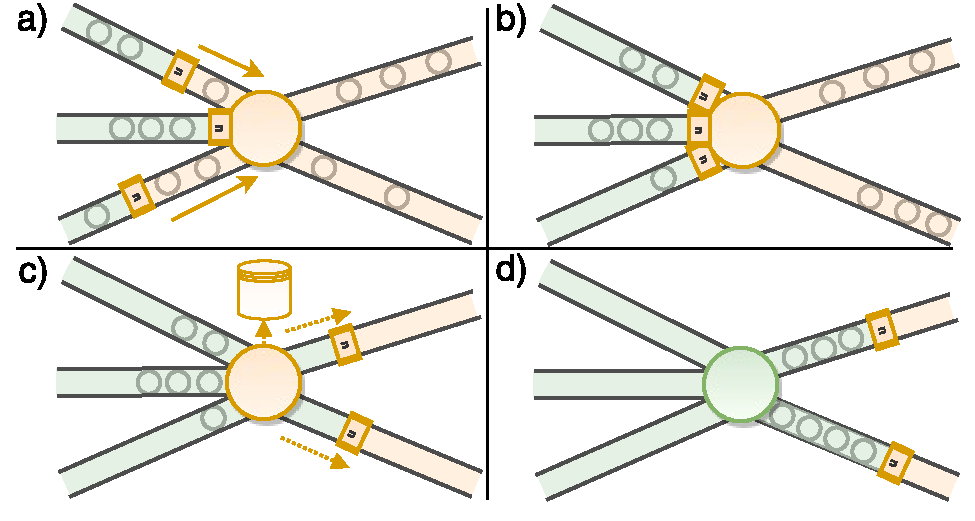
\includegraphics[width=\textwidth / 2]{figures/snapshots-highlights.pdf}
\caption{Alignment and Snapshotting Highlights.} 
\label{fig:snapshots-highlights}
\vspace{-2mm}
\end{figure}
\begin{figure}[t!]
\centering
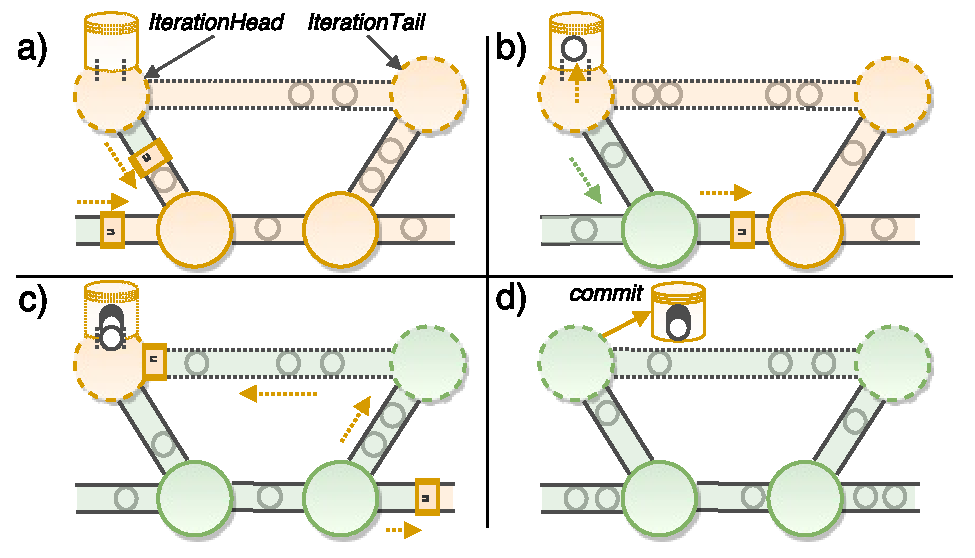
\includegraphics[width=\textwidth / 2]{figures/cycle-highlights.pdf}
\caption{Cycle Snapshotting Highlights.} 
\label{fig:cycle-highlights}
\vspace{-2mm}
\end{figure}


Let us consider only directed acyclic graphs (DAGs) for now. The protocol gets initiated at the source tasks of the dataflow by the \texttt{TaskManager}, however, for simplicity we assume here that the logic gets initiated upon receiving a special marker event in each and every task (sources would ``receive'' that first through a $Nil$ channel). \autoref{alg:snapdag} summarizes the snapshot alignment and pipelining protocol that executes when a marker is received. Mind that markers and records are handled sequentially by the same underlying thread that also invokes user-defined operators. 

\para{Alignment:} \autoref{fig:snapshots-highlights} vizualizes the steps prior to and during snapshotting in more detail. When a task receives a snapshot marker on one of its inputs, it blocks that channel since all computation associated with the current epoch has to finish before continuing further (\autoref{fig:snapshots-highlights}(a)). The blocking operation might result into spilling of in-transit records within that channel to disk, if allocated memory for network buffers reaches its limit. Once markers have been received in all inputs (\autoref{fig:snapshots-highlights}(b)) the task can further notify downstream tasks while also proceeding with snapshotting. Markers are first broadcasted forward and then local snapshotting is triggered, both of which can progress concurrently without sacrificing consistency (\autoref{fig:snapshots-highlights}(c)). Depending on the backend support, snapshots can be triggered and executed asynchronously by another thread, thus, minimizing their impact to the overall throughput. Once local snapshotting is initiated (\autoref{fig:snapshots-highlights}(d)) input channels are unblocked and regular operation continues to the next epoch. Overall, reliable FIFO data channels (Assumption II), combined with alignment guarantee that epoch-order is always respected. 

\para{Relaxing Consistency}: It is possible, if a pipeline allows for relaxed consistency requirements, to disable alignment (i.e., no input blocking). Essentially, this means that a snapshot on epoch $n$ will contain side-effects of input residing in epochs $\geq n$. Upon rollback records succeeding epochs $n$ are going to be ingested again, resulting into multiple state updates. This type of processing guarantees, also known as \emph{at-least-once processing}, can be enabled on Flink to trade-off consistency for practically zero latency impact if the application has no critical requirements.


\begin{algorithm}[h]
$inputs$ $\leftarrow$ configured\_inputs\;
$outputs$ $\leftarrow$ configured\_outputs\;
$blocked \leftarrow \emptyset$ \;
% $operator$ $\leftarrow$ dataflow\_operator\;

\Hdl{$\langle marker \rangle$ from $in \in inputs$}{
\If{$in \neq Nil$}{
 $blocked \leftarrow blocked \cup in$\;
 $in$.block()\;
}
\If{$blocked = inputs$}{
\ForEach{$out \in outputs$}{
$out$.send($\langle marker \rangle$)\;
}
triggerSnapshot()\;
\ForEach {$in \in inputs$}{
$in$.unblock()\;
}
$blocked \leftarrow \emptyset$ \;
}
}
\caption{Snapshot Alignment}
\label{alg:snapdag}
\end{algorithm}

\subsubsection{Dealing with Dataflow Cycles}

Dataflow graphs in Flink can also support cycles. Cycles are currently defined explicitly through Flink's programming API as asynchronous iterations, though bulk synchronous iterations (e.g., on stream windows) are also considered and can be supported in the future. Cyclic snapshotting is handled as a special case and implemented by system-specific, implicit tasks: an \texttt{IterationHead} and \texttt{IterationTail}. These tasks act as regular dataflow \emph{source} and \emph{sink} respectively, yet, they are collocated in the same physical instance to share an in-memory buffer and thus, implement loopback streams transparently.

The default stream alignment logic presented (\autoref{alg:snapdag}) would result into an incomplete distributed snapshot if applied on cyclic graphs. That is due to the fact that records belonging to prior epochs could still remain indefinitely in-transit within a cycle even after a snapshot has been taken over. Thus, it is crucial to persist these records in the snapshot in order to get a complete picture of the correct distributed execution \cite{chandy1985distributed,elnozahy2002survey}. Alternative approaches to this problem consider a ``flushing'' phase which enforces the inclusion of all the in-transit records to the internal state of each task \cite{jacques2016consistent}, however, we argue that this problem is only relevant to the state of a cycle. Thus, we execute a similar special logging protocol (\autoref{alg:snapcycle}) that runs solely within the \texttt{IterationHead} instances of each cycle.


As described in detail in \autoref{alg:snapcycle} and also visualized in \autoref{fig:cycle-highlights}, \texttt{IterationHead} tasks receive a special marker from the runtime signifying each epoch, same as the sources of the dataflow graph. At that instance, they disseminate markers further within a cycle and start logging in their own managed state all in-transit events that exist within a cycle in that respective partition (\autoref{fig:cycle-highlights}(a)). Once the marker of the snapshot is received back through their respective collocated \texttt{IterationTail} (\autoref{fig:cycle-highlights}(c)) they trigger a snapshot of that log containing a complete backup of all transmitted records in that epoch (\autoref{fig:cycle-highlights}(d)). Again, FIFO channels and alignment executed by the rest of the tasks within a cycle (\autoref{fig:cycle-highlights}(b)) ensures that no records from succeeding epochs will transit prior to the marker. This special logic also restricts channel logging to cycles and does not enforce anything other than task states to be included in the snapshot for the rest of the  graph.

%(unlike Chandy and Lamport's \cite{chandy1985distributed} algorithm or state-of-the-art protocols that focus on weakly connected dataflow graphs \cite{elnozahy2002survey,jacques2016consistent,murray2013naiad}).

\begin{algorithm}[t]
$outputs$ $\leftarrow$ configured\_outputs\;
$isLogging \leftarrow false$ \;
$log \leftarrow \emptyset$ \;

\Hdl{$\langle marker \rangle$}{
\eIf{$isLogging$}{
triggerSnapshot($log$) \;
$log \leftarrow \emptyset$ \;
$isLogging \leftarrow false$ \;
}{
$isLogging \leftarrow true$ \;
\ForEach{$out \in outputs$}{
$out$.send($\langle marker \rangle$)\;
}
}
}
\Hdl{$record$}{
\If{$isLogging$}{
 $log \leftarrow log \cup record$\;
}
\ForEach{$out \in outputs$}{
$out$.send($record$)\;
}
}
\caption{Snapshotting in Cycles}
\label{alg:snapcycle}
\end{algorithm}


\subsection{Usages and Consistent Rollback}

%\stephan{I would not even introduce the term "Savepoints" here, but simply stick with checkpoints/snapshots. More or less all checkpoints are externalized (at least in proper high availability setups). Mentioning that checkpoints can be explicitly archived for later rollback/reprocessing, etc makes sense. Other than that, I would simply mention that checkpoints define consistent points across parallel operators and thus are suitable points for reconfiguration. Reconfiguration conceptually happens via checkpoint/stop/modify/restore, but can also happen by attaching reconfiguration commands to barriers, which then reconfigure operators (replace code) at the point where the snapshot is taken. The later is not yet implemented (future work), but is worth mentioning in my opinion.}

Consistent snapshots, described previously in \autoref{sec:snapshots} form the basis for a variety of operations using the Apache Flink system. Periodic snapshots are automatically triggered by Flink's runtime as a form of per-job ``checkpoint'' for the purposes of consistent fail recovery whenever partial failures occur. However, the usages of snapshots go beyond fault tolerance needs. For a system that is widely deployed in a cloud infrastructure, having the ability to scale resources in or out and lease containers is nowadays a necessity. In principle, failover and re-scaling are two operations that share the same underlying need for consistent reconfiguration support \cite{castro2013integrating}. In this section we describe in more detail the operational benefits that distributed snapshots make feasible, as well as the rollback reconfiguration schemes that are currently supported.

\subsubsection{Snapshot Usages}
\label{sec:savepoints}

Flink's snapshots define consistent points across parallel operators and thus, are suitable points for reconfiguration. The metadata of a snapshot contains all necessary information required to retrieve the complete pipeline state from an associated durable storage backend such as references and indexes to operator state partitions (i.e., key-groups) and upstream logs (in case of cyclic graphs). Common causes of reconfiguration are: 1) application logic updates (e.g., software patches) of already running jobs by replacing operators accessing the same snapshotted state or adding new state entries instead and 2) application versioning, allowing forking running pipelines (an example depicted in \autoref{fig:savepoints}). In practice, reconfiguration follows a \texttt{checkpoint-stop-modify-restore} cycle, initiated externally by the user. However, it is also possible to be triggered topologically by attaching reconfiguration commands to snapshot markers which reconfigure operators (replace code) at the point where the snapshot is taken. 

\begin{figure}[t]
\centering
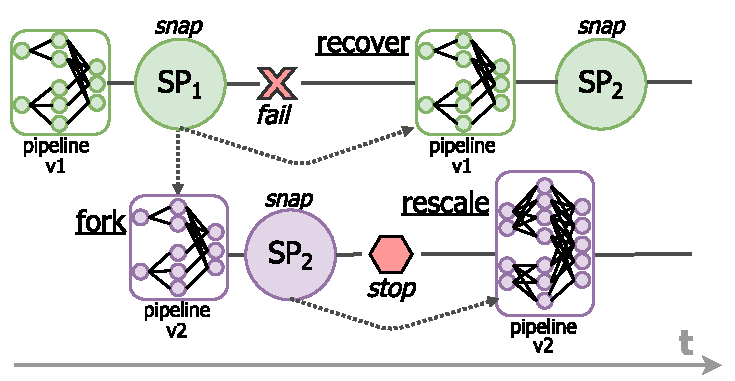
\includegraphics[width=\textwidth / 2]{figures/savepointsexamples.pdf}
\vspace{-6mm}
\caption{Snapshot usage examples.} 
\label{fig:savepoints}
\vspace{-4mm}
\end{figure}

%\paris{perhaps we could elaborate more here and add a motivating figure with snapshots and usages}
%\stefan{While savepoints and checkpoints are currently in the same format, we are planning to change this in the future. In particular, we are talking about costly features or properties, such as rescalability. We want to keep checkpoints as cheap as possible, at the cost of not supporting certain ops like rescaling from checkpoints. Savepoints, in turn, could be more costly but provide rescalability. Key-groups come with a certain cost, not only in meta data. Some backends may require some live partitioning before writing the snapshot. On top of that, key-groups can also mess with other natural groupings, such as namespaces that we find in windowing. For example, it would be nice to have locality for all keys in a window, so that we can quickly iterate over the window. However, we need to write data in key-group order, which forces us to split up the natural grouping of windows, into up to one partial window per key-group. Also in the context of incremental snapshotting, key-groups can easily become problematic. So checkpoints might support incremental snapshots, while savepoints might require full snapshots.}

\subsubsection{Consistent State Rollback}

Rollback recovery gets initiated upon a task failure or when there is a need to rescale. Typically, the latest snapshot is used to restart the application from the beginning of the latest committed epoch. Depending on the rollback cause, different recovery schemes are employed. For example. during a full restart or rescaling, all tasks are being redeployed, while after a failure only the tasks belonging to the affected connected component (of the execution graph) are reconfigured. In essence, known incremental recovery techniques from  micro-batch processing \cite{zaharia2012discretized} are orthogonal to this approach and can also be employed. A snapshot epoch acts as synchronization point, similarly to a micro-batch or an input-split. On recovery, new task instances are being scheduled and, upon initialization, retrieve their allocated shard of state. In the case of  \texttt{Iteration Head} recovery, all records logged during the snapshot are recovered and flushed to output channels prior to their regular record-forwarding logic. Eventually, all states within the pipeline are progressively retrieved and applied to reflect an exact, valid distributed execution at the restored epoch. 

%It is possible that a pipeline's dataflow graph consists of multiple weakly connected components. In case of a failure on a single of these connected components, rollback recovery can be applied only in the respective component, leaving other components' normal execution intact. This optimization yields a more fine-grained recovery scheme and does not violate consistency since there are no data dependencies across disconnected components. 

It is additionally required for all data sources to rollback input from the epoch where the snapshot occurred. Flink's data sources provide this functionality out-of-the-box by maintaining offsets to the latest record processed prior to an epoch from external logging systems. Upon recovery the aggregate state of those sources reflects the exact distributed ingestion progress made prior to the recovered epoch. This approach assumes that external logging systems, that sources communicate with, index and sequence data across partitions in a durable manner (e.g., Kafka, Kinesis, PubSub and Distributed File Systems). 

%\stephan{It is worth mentioning that techniques known from batch/mini-batch processing for incremental recovery are applicable here. The completed checkpoint is the point to restart from (similar to beginning of "input split" or beginning of "mini batch"). The only difference here is that downstream operators have to be rolled back as well, for exactly-once semantics (or not, for at-least-once semantics).}
%\paris{Maybe explain briefly how unreliable sources can work}

%Alternatively each data source instance has to maintain a durable write-ahead-log 
%of all uncommitted input and delay ingestion by an epoch to emulate the same assumptions through Flink's snapshotting mechanism.





%!TEX root = main.tex


\section{Implementation and Usage}

With explicit managed state and a pipelined snapshotting algorithm at its core, Flink maintains a rich ecosystem of backends, connectors and other services that interplay seamlessly and enrich further the capabilities of its global state establishment mechanism. In this section we summarize how each of these subsystems builds on-top of Flink's core architecture, while expanding it with asynchronous communication, delivery guarantees and external state querying support.

\label{sec:implementation}

\subsection{State Backend Support}

Managed state consistency is coordinated by Flink's snapshotting algorithm (\autoref{sec:snapshots}), however, state access and persistence are the main concerns of the state backend module. There are currently three different backends supported by the Flink stack : 1) \emph{In-Memory}, 2) \emph{File-Based} and 3) \emph{Out-of-Core}. Depending on the overall expected managed state accumulated in a pipeline, each of the backends offers a suitable trade-off between execution throughput, scalability and flexibility.

\para{In-Memory}
The \emph{In-Memory} backend maintains active managed state in local, allocated heap space and snapshotted state within the Job Manager's heap space. This is, in some distinct use-cases, a preferable choice that yields very high throughput. For example, pipeline testing and debugging or actual deployments with low state capacity requirements such as filtering and basic ETL can make a reasonable use of this backend. Upon each task's \texttt{triggerSnapshot()} invocation local state is serialized, copied and transfered to the Job Manager together with typical snapshot metadata. As a result, the Job Manager needs to have enough heap space allocated in order to be able sustain all physical task materialized states for each snapshot.

\para{File-Based:}
In most cases, complete pipeline snapshots involve much larger active managed state than what can fit in memory of a single node. The \emph{File-Based} backend leaves distributed uncommitted state in heap space, however, whenever snapshotting is invoked the state is being copied from heap to a configured distributed file system directory (e.g., HDFS). As a result, snapshot metadata is also kept to a minimum (containing mainly file references), while throughput can remain high since operations on uncommitted memory happen in-place at the local heap.

\para{Out-of-Core:}
Complex pipelines often need to maintain very large managed state such as Terabytes of indexes and large sequences of sliding windows upon which user-defined logic can operate continuously. In such cases, local heap space is insufficient to maintain even locally accessed active state, especially for certain task operators (e.g., Flink's \texttt{WindowOperator}). Flink provides an \emph{out-of-core} backend that decouples state operations performed on each task from the physical location where state itself is persisted and updated. In its current implementation, out-of-core state is interfaced with an embedded file-backed key-value database (i.e., RocksDB). Therefore, state capacity is only limited by the file system space allocated at the host where this backend is deployed. Moreover, operations triggered on managed state such as \texttt{update} for mutable state and \texttt{add} for append-only \texttt{ListState} are carried over to the embedded key-value store instead. One of the benefits that are enabled out-of-the-box with such a scheme is that most per-key operations can be executed asynchronously at the backend without sacrificing throughput. On the other hand, state value retrievals can take more time to complete, especially if some specific state has to be retrieved from compacted files on disk and it is no longer within the backend's memory. \paris{@stefan please add or correct whatever you see fit. You know this part better than anyone else.}

\subsection{Asynchronous Snapshots and Notifications}
\label{sec:async}
One of the advantages of the pipelined snapshotting protocol presented in \autoref{sec:snapshots} is that it does not restrain the actual acquisition of snapshots to be synchronous. A call of \texttt{triggerSnapshot()} by each task is expected to create an identical copy of the current state of that task. In case there is support by a backend module to execute this operation asynchronously, it can be used without violating consistency. The \emph{out-of-core} backend of Flink offers the capability to trigger snapshots in a purely asynchronous way by copying the full compacted key-value database to a backup directory by another thread, thus, letting normal processing proceed without interruptions. Once local snapshotting operations have been completed the notifications are triggered back at the tasks and carried out to the \emph{JobManager} alongside associated meta-data where a full snapshot can be declared as complete. Asynchronous snapshotting also unlocks the possibility to multiplex multiple instances of the protocol running at the same time in a dataflow graph. That means that while for example a periodic snapshot is undergoing, a user can also trigger a savepoint and both of the associated snapshots will run concurrently and distributively, each invoking its own asynchronous state copy and epoch.

Another feature that is provided to tasks as an optional asynchronous subscription-based mechanism is to trigger notifications about completed snapshots back at the tasks that request them. This is especially useful for garbage collection, discarding write ahead logs or for executing output commit protocols as we explain further in \autoref{sec:outputcommit}.

\subsection{Queryable State}

A recent, yet notable addition among Flink's state management mechanisms, is the ability to execute selective ad-hoc queries on managed state from outside the system. Continuous data stream processing pipelines often build and maintain partitioned state inside operators that could be potentially harnessed at any time and used to provide fast, actionable knowledge, in a similar fashion to in-memory database usage \cite{kipfanalytics}. Queryable state allows for any declared managed state within a pipeline, currently scoped by key, to be accessed outside the system for asynchronous reading, through a subscription-based API. First, managed state that allows for query access is declared in the original application. Upon state declaration, introduced in \autoref{sec:managedstate}, it is possible to allow access from external queries by simply setting a flag in the descriptor that is used to create the actual state, having an assigned unique name for this specific state to be accessed, as such:

\begin{lstlisting}[language=scala]
//stream processing application logic
val descriptor: ValueStateDescriptor[MySchema] = ...
descriptor.setQueryable("myKV")
...
val mutState: ValueState[MySchema] = ctx.getState(descriptor)
\end{lstlisting}

\para{} Upon deployment, a state registry service gets initiated and runs concurrently with the operator holding write access to that state. A client that wishes to read this state can, at any time submit an asynchronous query (obtaining a \texttt{future}) to that service, specifying the job id, registered state name and the key under which the state is active, as shown below:

\begin{lstlisting}[language=scala]
//client logic
val client = QueryableStateClient(cfg);
var readState: Future<?> = client.getKVState(job, "myKV", key);
MyDeserializer[MySchema](Await.result(readState, timeout));
\end{lstlisting}

The current implementation of queryable state allows for retrieving and sending, internally through Akka messaging, copies of serialized state values straight from the operator heap memory or the backend store in case of out-of-core state. Despite current limitations to point lookups of the current value (\texttt{ListState} is not yet supported as of Flink v1.2.0) the ability to access state generalizes the usages of a stream processor, beyond the needs of data transformation or application logic needs and adds further potential for ad-hoc data analysis. From a traditional database isolation-level viewpoint, this feature also includes the ability to access and operator on uncommitted state, thus, allowing for a more relaxed, yet highly accessible \emph{read-uncommitted} read isolation, compared to already provided \emph{read-committed} read isolation guaranteed by its specialized sinks through its snapshotting mechanism (see \autoref{sec:outputcommit}).

\subsection{Output Commit}
\label{sec:outputcommit}

So far we have considered consistency guarantees associated with the internal state of the system. However, it is most often important to offer guarantees regarding the side effects that a pipeline leaves to the outside world, whether that is a distributed database, file system or message queue. A pipeline interfaces with the outside world mainly via its dataflow sinks. Thus, it is often crucial that sinks can offer exactly-once delivery guarantees. The feasibility of achieving ``read-committed'' isolation guarantees to external writes depends on the properties of the system upon which sinks commit output and typically comes at a higher latency cost that can, at-times, violate strong SLAs on latency. A pipeline can always be halted between snapshots after a failure or an urgent reconfiguration request and both input and state can be rolled back consistently, as it was described in \ref{sec:core}. However, the same cannot always be guaranteed about the output. If sinks are connected, for example, to a printer that instantly flushes data on paper, a rollback would possibly print the same or alternating text twice. Flink's programming model is equipped with two main types of sinks that facilitate ``read-committed'' output and build on the snapshotting mechanism: the 1) Idempotent Database Sink and 2) Bucketing File Sink.

\para{Idempotent Database Sink: } Idempotency is a property used extensively by several systems at the presence of failures in order to encourage repeatability and alleviate bookkeeping efforts and complex decision protocols to offer delivery guarantees\cite{CUSTOM:web/SparkStructuredStreaming,millwheel}. Flink's database sink executes user-defined, idempotent database queries to a distributed database for each input received per parallel sink. Deterministic streams (that do not involve stream interleaving or other forms of non-determinism) can rely on that sink to operate consistently with the database. However, in most cases where deterministic processing cannot be guaranteed, a write-ahead log of prepared query statements is kept as part of the state of that sink and maintained per-epoch. Once an asynchronous notification (\autoref{sec:async}) arrives regarding a completed epoch snapshot, the database sink commits all pending writes to the database at the expense of additional output latency (for a snapshot to complete and its notification to arrive to the sinks). Query idempotency guarantees that even failures during committing can be resolved by simply re-committing the same queries and thus, eventually, leaving the same side effects upon subsequent system reconfigurations. \paris{what are the database properties required and why is it only cassandra based?}

\begin{figure}[t!]
\centering
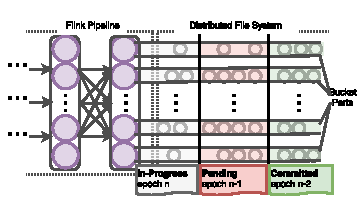
\includegraphics[width=\textwidth / 2]{figures/filecommit.pdf}
\caption{A visualization of Bucketing File Sinks.} 
\label{fig:filecommit}
\vspace{-4mm}
\end{figure}

\para{Bucketing File Sink: } Committing state to a distributed file systems (e.g. HDFS) has to be made in a coordinated way since a file has to be consistent across all its file partitions. Flink's bucketing file sink (depicted in \autoref{fig:filecommit}) eliminates the need for a write-ahead log and eagerly appends stream output within uncommitted distributed file directories which group (or ``bucket'') partition parts by time-period. After a pre-configured inactivity time-period \texttt{in-progress} directories become \texttt{pending} and are ready to be committed. The Bucketing File Sink integrates with Flink's snapshotting algorithm and associates epochs with buckets. Once a file bucket is under \texttt{pending} mode and an asynchronous notification for an associated epoch has been received, it can be moved to a \texttt{committed} state via a \texttt{rename} operation. Potential disruptions between epochs resolve into a \texttt{truncate} (Posix) operation, which is currently supported by major distributed file systems and conveniently reverses append operations. \paris{i guess the non-truncate approach is ugly. Should we write about it?}

\subsection{Asynchronous IO}
\paris{Maybe we can simply highlight how this operates and aligns with the snapshotting protocol}

\subsection{High Availability \& Reconfiguration}
\paris{This is just an implementation specific problem. We should mention how we utilized zookeeper and offer some insights about what metadata we store since it is useful for many people actually.}

	

%!TEX root = main.tex


\section{Large-Scale Deployments}

\kostas{We probably do not need a traditional evaluation section but rather some numbers from King, Alibaba etc. taken from really large deployments with terabytes of managed state}

\paris{We can also benchmark and collect stats for the following pipeline impact factors: 1) state size (small and large state), 2) alignment (no snapshot - at least once - exactly once), 3) job graph length -> snapshot latency - worse recovery (rollback earlier). Ultimately, it is nice to show the costs of EtE, Snapshot  and Recovery Latency. 
We can probably include at least once cyclic graph as well.
}

%!TEX root = main.tex

\section{Related Work}
\label{sec:related}

\para{Reliable Dataflow Processing: } Flink offers coarse grained, job-level snapshot maintance which offers various operational benefits. Several proposed reconfiguration and state management schemes \cite{castro2013integrating} are often restricted to fine-grained task management and reconfiguration, thus, lacking the benefits, applications and scale of global snapshots \autoref{sec:savepoints}.

IBM Streams employs a pipelined checkpointing mechanism \cite{jacques2016consistent} that executes in-flight with data streams as with Flink's, tailored to weakly connected graphs with potential cycles. The most distinct difference to Flink's approach is that IBM Stream coordinates a two-phase protocol as such: 1) First, all records in transit are consumed in order to make sure that they are reflected in the global state while blocking all outputs. 2) All operators trigger their snapshot in topological order, using markers as in our technique and resume normal operation. Flink's protocol restricts draining solely within cycles without affecting regular processing whatsoever. Furthermore, Flink's alignment is a local operation and does not halt global progress or hold up output in an execution graph, thus it is more transparent and non-intrusive. Finally, IBM Streams supports language abstractions for selective fault tolerance. On Flink, the choice of snapshotting state is achieved through simply using managed state versus unregistered state, without requiring further user intervention. In the scope of a pipeline/component, snapshots can also be enabled or disabled through Flink's configuration. 

Apache Storm \cite{CUSTOM:web/Storm} initially offered solely guaranteed record processing through a form of event sourcing using record dependency tracking. However, the most recent releases incorporated Flink's algorithm to its core \cite{CUSTOM:web/stormsux} in order to support exactly-once processing guarantees. Meteor shower \cite{wang2012meteor} employs an similar alignment phase to Flink. However, it cannot incorporate cyclic dataflow graphs which is a common case for online machine learning \cite{de2015samoa} and other applications. Furthemore, source upstream backup introduces heavy ingestion latency costs and is not necessary when input streams are peristed within durable logs \cite{kreps2011kafka}. The same solution does not cover state rescaling and transparent programming model concerns. Naiad \cite{murray2013naiad} and the sweeping checkpointing technique [15] enforce in-transit state logging even in subgraphs where cycles are not present. Furthermore, Naiad's proposed three phase commit disrupts the overall execution for the purpose of snapshotting. 

Finally, Millwheel \cite{millwheel} offered a complete solution to end-to-end processing guarantees, similarly to Flink. However, its heavy transactional nature, idempotency constraints and strong dependence on a high write-throughput, always-available, replicated data store \cite{chang2008bigtable,corbett2013spanner} makes this approach unfordable in commodity deployments. In fact, Apache Flink serves today as a feature-complete runner of Apache Beam, Google's open-source implementation of the Dataflow Model\cite{CUSTOM:web/Dataflow}.

\para{Microbatching}: Stream micro-batching or batch-stream processing (e.g. Spark Streaming \cite{zaharia2012discretized}, Comet \cite{he2010comet}) emulates continuous, consistent data processing through a recuring deterministic batch processing operations. In essense, this approach assigns distinct epochs of a stream to be scheduled independently. Fault tolerance and reconfiguration is guaranteed out-of-the-box through reliable batch processing at the cost of high reconfiguration latency and restrictive, programming model limited to incremental, deterministic set operations. Trident \cite{CUSTOM:web/trident}, a higher level framework built on Apache Storm offered exactly-once processing guarantees through a similar transactional approach on predefined sets but executed on long-running data stream tasks. While fault tolerance is guarnateed with such techniques, we argue that high latency and such programming model restrictions make this approach non-transparent to the user. 


%!TEX root = draft.tex

\section{Acknowledgments}

%!TEX root = main.tex

\section{Conclusion and Future Work}
\label{sec:conclusion}

We presented Apache Flink's core mechanisms for managing persistent, large-scale pipelines with large application state in production. Flink is a flexible, reconfigurable distributed system which runs continuous, analytical, data-centric computation offering strong state consistency guarantees. A distinct snapshotting mechanism acquires a global view of the system periodically or upon demand which allows for coarse grained rollback recovery in a asynchronous, transparent and efficient manner. Snapshots allow for fundamentally practical reconfiguration usages, ranging from partial failure recovery to application versioning, debugging and general state management. Managed state in Apache Flink can be trivially declared through special collections that abstract runtime state management concerns from the programmer. We demonstrated Flink's practical impact with large-scale deployment measurements with terabytes of state, continuously updated by transformations triggered by millions of continuous streams of input data.

\para{Future Work:} Our main future focus on Apache Flink is to improve further its state management capabilities with asynchronous main memory state and incremental snapshots, enabling automated system estimation of throughput and reconfiguration latency trade-offs. Furthermore, we are planning to include the capability of auto-scaling pipelines according to runtime requirements without user circumvention. Finally, we want to support deeper stateful analytics through efficient structured iterative processing, one of the biggest challenges in continuous processing today.

\para{Acknowledgments:} We would like to thank all reviewers who gave us valuable feedback and the whole community of Flink's committers and contributors who offered ideas and code to the system. 

\balance
%\Urlmuskip=0mu plus 2mu\relax




\renewcommand\baselinestretch{0.99}
{
\small
\bibliographystyle{abbrv}
\bibliography{main}
}

%\bibliographystyle{abbrv}
%\bibliography{main}  


%APPENDIX is optional.
% ****************** APPENDIX **************************************
% Example of an appendix; typically would start on a new page
%pagebreak

%\begin{appendix}
%\end{appendix}


\end{document}
